\section{Materials and Methods}
\label{sec:methods}

This section describes the experimental methodology used to evaluate computational efficiency and reconstruction fidelity across neural rendering architectures under sparse-view conditions. Figure~\ref{fig:pipeline} illustrates the three stages of the pipeline: (i) dataset preparation and sparse-view sampling; (ii) model configuration across generalizable adaptation and per-scene training regimes; and (iii) quantitative and qualitative evaluation on held-out views.

\begin{figure}[!t]
\centering
\resizebox{0.9\linewidth}{!}{%
\begin{tikzpicture}[
  >=stealth,
  block/.style={
    rectangle, draw=black!30, thick, fill=white,
    minimum width=4.1cm, minimum height=0.95cm,
    text centered, rounded corners=3pt, font=\tiny,
    align=center
  },
  line/.style={draw, thick, black!45, ->, >=stealth, rounded corners=2pt}
]

% --- LEVEL 1 & 2: Dados Iniciais ---
\node[block] (data) at (0, 0) {
  \textbf{\faDatabase\ Dataset} \\[0.5mm] 
  LLFF ($8$ scenes, $504 \times 378$)
};

\node[block] (split) at (0, -1.45) {
  \textbf{\faProjectDiagram\ Split Generation} \\[0.5mm] 
  Uniform \& Random (seed 42, $N \in \{3, 6, 10\}$)
};
\draw[line] (data.south) -- (split.north);


% --- LEVEL 3: Bifurcação dos Modelos ---
\node[block] (gen_models) at (-2.3, -3.1) {
  \textbf{\faBrain\ Generalizable Models} \\[0.5mm] 
  PixelNeRF $\cdot$ GNT
};

\node[block] (ps_models) at (2.3, -3.1) {
  \textbf{\faCogs\ Per-Scene Models} \\[0.5mm] 
  Instant-NGP $\cdot$ Nerfacto $\cdot$ Splatfacto
};

% Setas do Split para os Modelos
\draw[line] (split.south) -- ++(0,-0.32) -| (gen_models.north);
\draw[line] (split.south) -- ++(0,-0.32) -| (ps_models.north);


% --- LEVEL 4: Regimes de Treino ---
\node[block] (gen_reg) at (-2.3, -4.55) {
  \textbf{\faTasks\ Regimes} \\[0.5mm] 
  Zero-Shot, Fine-Tuning ($500$ steps)
};

\node[block] (ps_reg) at (2.3, -4.55) {
  \textbf{\faTasks\ Regime} \\[0.5mm] 
  Per-Scene ($N=10$, $30\text{k}$ steps)
};

% Setas dos Modelos para os Regimes
\draw[line] (gen_models.south) -- (gen_reg.north);
\draw[line] (ps_models.south) -- (ps_reg.north);


% --- LEVEL 5 & 6: Avaliação e Métricas ---
\node[block] (eval) at (0, -6.2) {
  \textbf{\faVial\ Evaluation} \\[0.5mm] 
  Unified Protocol (\texttt{llffhold=8})
};

% Setas dos Regimes convergindo para Avaliação
\draw[line] (gen_reg.south) -- ++(0,-0.32) -| ([xshift=-2.5mm]eval.north);
\draw[line] (ps_reg.south) -- ++(0,-0.32) -| ([xshift=2.5mm]eval.north);

\node[block] (metrics) at (0, -7.65) {
  \textbf{\faChartBar\ Metrics} \\[0.5mm] 
  \textbf{Qual:} PSNR, SSIM, LPIPS \ $|$ \ \textbf{Perf:} Time, FPS, VRAM
};
\draw[line] (eval.south) -- (metrics.north);


% --- BACKGROUND (Ambiente Isolado) ---
\begin{scope}[on background layer]
  \node[draw=black!20, dashed, fill=black!2, rounded corners=5pt, 
        inner xsep=12pt, inner ysep=15pt, 
        fit=(data)(split)(gen_models)(ps_models)(gen_reg)(ps_reg)(eval)(metrics),
        label={[anchor=south east, font=\scriptsize\color{black!60}]south east:
        {\faDocker} Docker \ $|$ \ NVIDIA GTX 1660S \ $|$ \ CUDA 12.6}] (env) {};
\end{scope}

\end{tikzpicture}%
}
\caption{Proposed benchmarking pipeline. COLMAP-calibrated sparse splits ($N \in \{3, 6, 10\}$) were evaluated across two architectural branches inside an isolated Docker environment: generalizable models under Zero-Shot and five fine-tuning strategies, and per-scene baselines trained to convergence, assessed via visual fidelity (PSNR, SSIM, LPIPS) and computational metrics (Time, FPS, VRAM).}
\label{fig:pipeline}
\end{figure}


\subsection{Dataset \& Splits}
\label{sec:data}
All experiments were conducted on the Local Light Field Fusion (LLFF) dataset \cite{mildenhall2019locallightfieldfusion}, which contains 8 forward-facing real-world scenes with COLMAP-calibrated camera poses and depth bounds, downscaled by a factor of 8 ($504 \times 378$ pixels). Following the few-shot evaluation protocol of Niemeyer et al.\ \cite{niemeyer2022regnerf}, every 8th image (\texttt{llffhold=8}) was reserved for testing, while the training subsets were restricted to $N \in \{3, 6, 10\}$ views. Two view selection criteria were compared on the \textit{fern} scene ($N=10$, Table~\ref{tab:split}): (i) \textit{Uniform}, where training views were sampled by linear interpolation over the dataset indices along the camera trajectory; and (ii) \textit{Random}, where views were drawn using a fixed seed (\texttt{seed=42}). Uniform sampling yielded higher PSNR across all tested models (up to $+0.54$ dB on PixelNeRF and $+0.15$ dB on GNT) and was therefore adopted for all remaining experiments.

\begin{table}[!t]
\centering
\caption{Comparison between uniform and random training view selection under $N=10$ views on the \textit{fern} scene. Uniform sampling along the camera trajectory improved reconstruction metrics across both generalizable and per-scene models.}
\label{tab:split}
\scriptsize
\begin{tabular*}{\linewidth}{@{\extracolsep{\fill}}llcccc}
\toprule
Model & Split & PSNR $\uparrow$ & SSIM $\uparrow$ & LPIPS $\downarrow$ & $\Delta$PSNR \\
\midrule
\multirow{2}{*}{PixelNeRF}
  & Uniform   & 6.98   & 0.047    & 0.846    & \multirow{2}{*}{\textbf{+0.54}} \\
  & Random    & 6.44   & 0.042    & 0.840    &                        \\
\midrule
\multirow{2}{*}{GNT}
  & Uniform   & 10.34  & 0.179    & 0.738    & \multirow{2}{*}{+0.15} \\
  & Random    & 10.19  & 0.184    & 0.742    &                        \\
\midrule
\multirow{2}{*}{Instant-NGP}
  & Uniform   & \textbf{13.57} & \textbf{0.231} & \textbf{0.627} & \multirow{2}{*}{+0.06} \\
  & Random    & 13.51  & 0.229    & 0.630    &                        \\
\midrule
\multirow{2}{*}{Nerfacto}
  & Uniform   & 12.04  & 0.227    & 0.809    & \multirow{2}{*}{+0.11} \\
  & Random    & 11.93  & 0.226    & 0.865    &                        \\
\bottomrule
\end{tabular*}
\end{table}

Standardized execution parameters were applied across the benchmark. Camera pose refinement was disabled in Nerfacto because equivalent pose optimization is not natively supported by the other evaluated architectures. Mixed-precision training was enabled for all models, and the hash table capacity in Instant-NGP and Nerfacto was set to $2^{16}$ with white background compositing. For GNT, structural hyperparameters were kept at 48 coarse and fine samples per ray, a transformer depth of 8, and a feature width of 64 \cite{t2023attentionnerfneeds}.

\subsection{Models \& Training Regimes}
\label{sec:regimes}
Five representative architectures were evaluated across two modeling groups: generalizable implicit networks (PixelNeRF \cite{yu2021pixelnerfneuralradiancefields} and GNT \cite{t2023attentionnerfneeds}) and per-scene baselines comprising implicit hash grids (Instant-NGP \cite{muller2022} and Nerfacto \cite{Tancik2023}) and explicit 3D Gaussian primitives (Splatfacto \cite{kerbl3Dgaussians}). Three operational regimes were defined: (i) \textit{Zero-Shot (ZS)}, where pre-trained generalizable weights were evaluated directly without gradient updates; (ii) \textit{Fine-Tuning (FT)}, where pre-trained generalizable models were adapted on sparse target views; and (iii) \textit{Per-Scene}, where baseline representations were trained from scratch on $N=10$ views for $30,000$ iterations.

\subsubsection{Fine-Tuning Strategies and Implementation}
Custom Nerfstudio wrapper packages (\texttt{nerfstudio-gnt} and \texttt{nerfstudio-pixelnerf}\footnote{Repositories and packages: \url{https://github.com/Felipe-gsilva/Few-Shot-NeRFs/} and \url{https://github.com/Felipe-gsilva/nerf-ann-paper/}.}) were implemented with a shared adaptation module (\texttt{adaptation.py}) to execute the five strategies described in Section~\ref{sec:ft_theory}.

During model initialization, \texttt{setup\_adaptation()} configured the \texttt{requires\_grad} flags of each sub-network and replaced targeted projection layers. Under \textit{Full-FT}, gradient updates were enabled across both the 2D encoder and the 3D rendering network. Under \textit{PFT-Decoder}, the 2D feature encoder (\texttt{feature\_net} in GNT and \texttt{encoder} in PixelNeRF) was frozen and locked in evaluation mode (\texttt{.eval()}), restricting weight updates to the volumetric decoder (\texttt{net\_coarse}/\texttt{net\_fine} in GNT and \texttt{mlp\_coarse}/\texttt{mlp\_fine} in PixelNeRF). Under \textit{PFT-Backbone}, gradients were enabled only in the 2D encoder while all volumetric rendering layers remained frozen. For \textit{BitFit}, multidimensional weight tensors were frozen and gradients were restricted to 1D bias vectors (\texttt{name.endswith(".bias")}), corresponding to less than $0.15\%$ of the model parameters. For \textit{PEFT-LoRA}, the base model was frozen and linear projections (\texttt{q\_proj}, \texttt{v\_proj}, and MLP layers) were replaced with \texttt{LoRALinear} modules containing trainable rank-$r$ matrices $A \in \mathbb{R}^{r \times d_{\text{in}}}$ (Kaiming-uniform initialization) and $B \in \mathbb{R}^{d_{\text{out}} \times r}$ (zero initialization), scaled by $\alpha/r$.

Because Nerfstudio registers separate optimizer parameter groups for the 2D encoder and 3D renderer, freezing an entire sub-network produces an empty parameter list in PyTorch. This issue was handled by inserting an inert scalar tensor (\texttt{dummy\_param} with \texttt{requires\_grad=False}) into empty groups and overriding \texttt{model.train()} to prevent BatchNorm statistics from updating inside frozen encoders. Before test-view evaluation, \texttt{merge\_lora\_weights()} folded the low-rank increment $\Delta W = \frac{\alpha}{r}BA$ directly into the base weight matrix $W_0$ in-place, avoiding additional matrix multiplications during inference.

\subsubsection{Stratified K-Fold Grid Search and Convergence Calibration}
Hyperparameter sensitivity and variance across seeds were evaluated using a Stratified $K$-Fold protocol ($K=4$) over all eight LLFF scenes. Each fold paired a foliage scene with a structured indoor or architectural scene: Fold 0 (\textit{fern}, \textit{fortress}), Fold 1 (\textit{flower}, \textit{horns}), Fold 2 (\textit{leaves}, \textit{room}), and Fold 3 (\textit{orchids}, \textit{trex}). The search grid covered learning rates $\eta \in \{10^{-4}, 5\times 10^{-4}, 10^{-3}\}$ and LoRA ranks $r \in \{4, 8\}$ ($\alpha = 2r$) across three random seeds $\{42, 123, 999\}$ under $N=3$ input views, optimized with Adam (512 training rays and 128 evaluation rays per batch). Optimization runs that diverged on dense foliage scenes (producing $0.0$ dB PSNR on \textit{leaves} and \textit{orchids}) were excluded from the aggregated averages.

The number of fine-tuning iterations for the grid search was selected through an ablation experiment from $0$ to $30,000$ steps ($\{0, 100, 250, 500, 1\text{k}, 1.5\text{k}, 2\text{k}, 2.5\text{k}, 5\text{k}, 10\text{k}, 20\text{k}, 30\text{k}\}$) on the \textit{fern} scene ($N=3$), shown in Figure~\ref{fig:ft_steps_ablation}. Four distinct convergence trajectories were observed: (i) \textit{PixelNeRF (PFT-Backbone, $\eta=10^{-4}$)} increased from $5.72$ dB (ZS) to its peak between $500$ and $1,000$ steps ($11.03\text{--}11.53$ dB PSNR), after which continued training caused overfitting and reduced PSNR to $7.85$ dB at $10\text{k}$ and $7.63$ dB at $20\text{k}$ steps; (ii) \textit{PixelNeRF (PEFT-LoRA, $r=4, \eta=10^{-3}$)} reached its highest PSNR at $100$ steps ($9.89$ dB) and its lowest LPIPS at $5,000$ steps ($0.714$), followed by representation degradation beyond $10,000$ steps ($4.70$ dB PSNR and $0.0004$ SSIM at $20\text{k}$); (iii) \textit{GNT (PFT-Backbone, $\eta=10^{-4}$)} remained nearly constant ($\approx 10.19\text{--}10.33$ dB) across all $30,000$ steps, indicating that updating the 2D patch embedder alone did not alter epipolar ray aggregation; and (iv) \textit{GNT (PEFT-LoRA, $r=4, \eta=10^{-3}$)} reached $14.29$ dB by $500$ steps ($\sim 92\%$ of its $15.59$ dB PSNR peak at $10,000$ steps) and continued improving structural similarity and LPIPS up to $20\text{k}\text{--}30\text{k}$ steps ($0.359$ SSIM and $0.675$ LPIPS), with a slight PSNR drop at $30\text{k}$ ($14.51$ dB). Based on these curves, $500$ steps was adopted as the standard iteration budget for the $K$-Fold grid search, avoiding overfitting in PixelNeRF while retaining over $90\%$ of GNT's peak gain within $\sim 50\text{ s}$.

\begin{figure*}[!t]
\centering
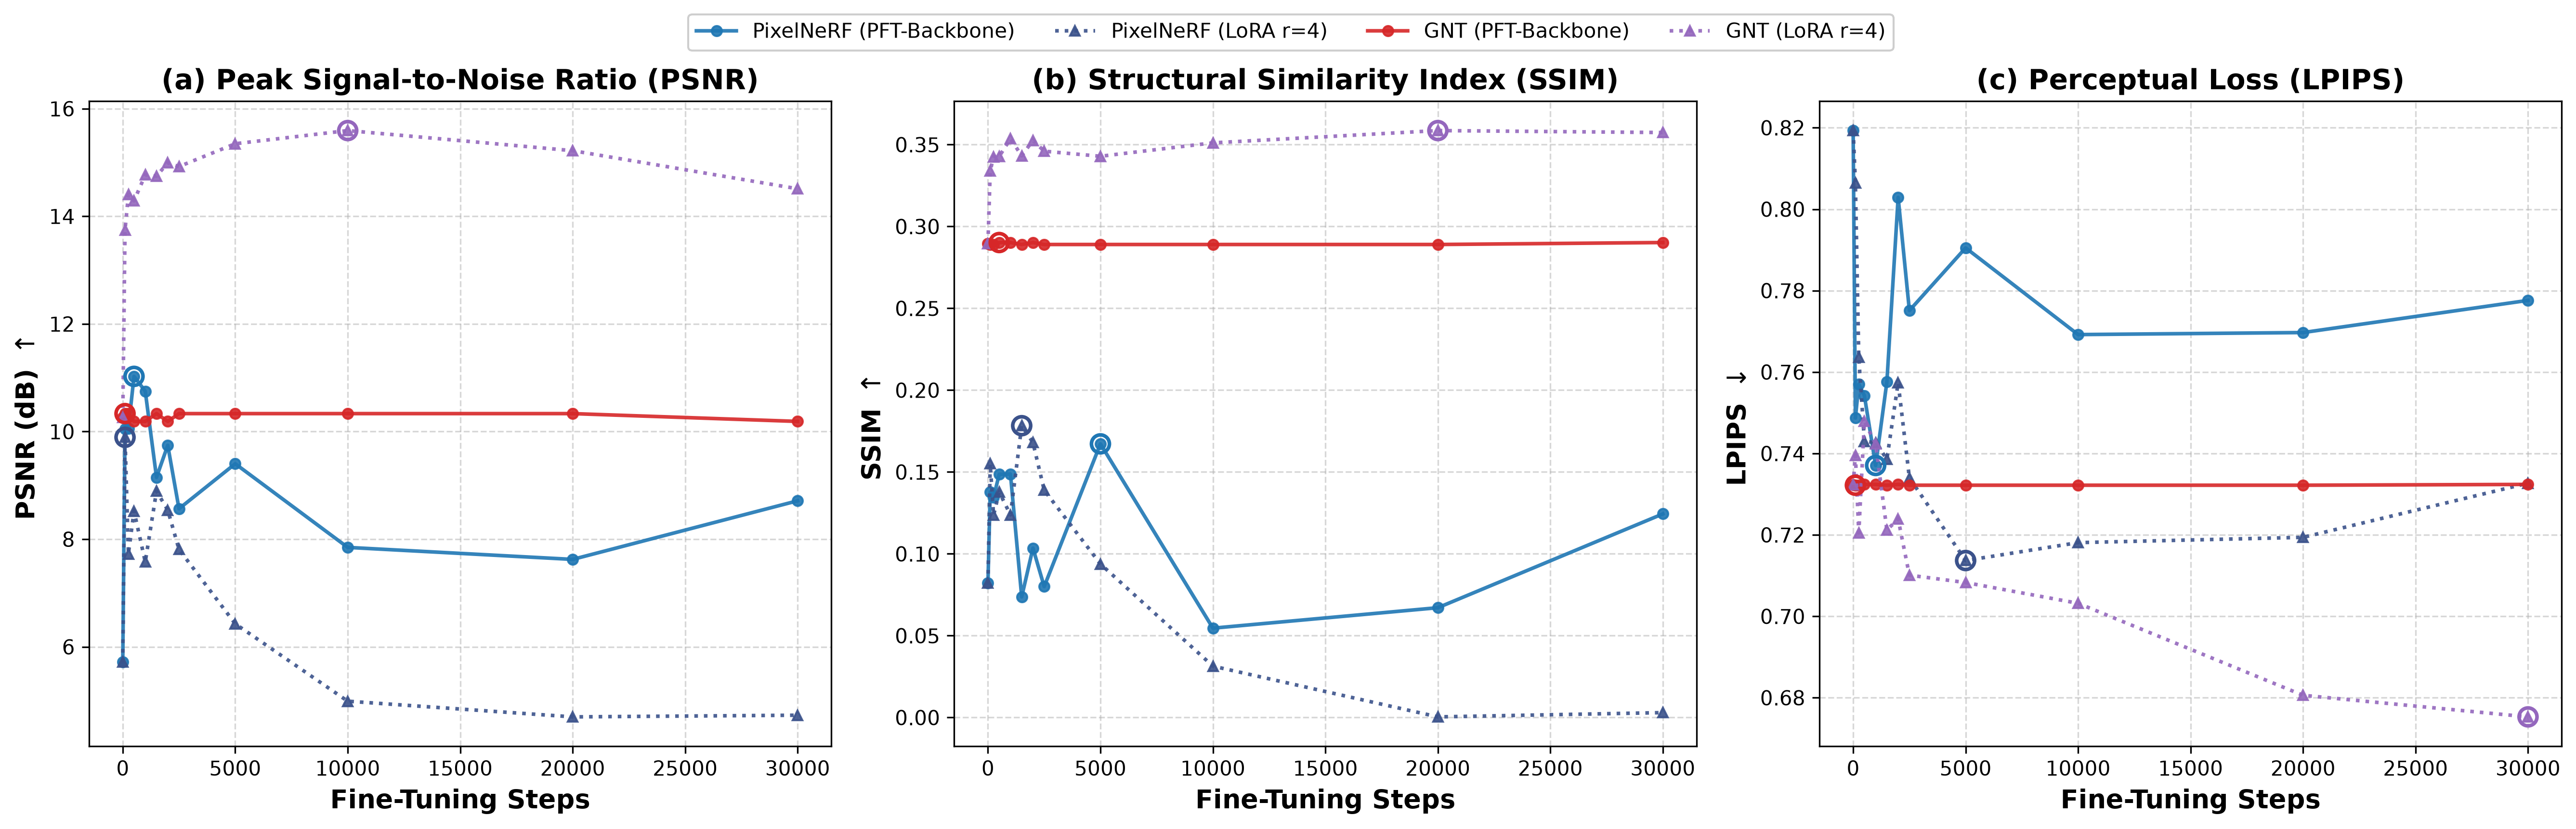
\includegraphics[width=0.88\textwidth]{img/ft_steps_ablation.png}
\vspace{-3pt}
\caption{Ablation of fine-tuning iterations from $0$ (Zero-Shot) to $30,000$ steps on the \textit{fern} scene ($N=3$) for (a) PSNR, (b) SSIM, and (c) LPIPS; circled points mark global optima. PixelNeRF reached its peak between $500$ and $1,000$ steps before degrading due to overfitting ($4.70$ dB under LoRA at $20\text{k}$ steps), whereas GNT with PEFT-LoRA ($r=4$) obtained $>91\%$ of its maximum PSNR gain by $500$ steps ($14.29$ vs.\ $15.59$ dB at $10\text{k}$) and remained stable up to $30\text{k}$ steps.}
\label{fig:ft_steps_ablation}
\end{figure*}

\subsection{Evaluation \& Metrics}
\label{sec:metrics}
All evaluations were executed on the held-out test views (\texttt{llffhold=8}) inside isolated NVIDIA Docker containers using an NVIDIA GeForce GTX 1660 Super GPU (6GB VRAM, CUDA 12.6). Reconstruction quality was measured using PSNR, SSIM \cite{wang2004image}, and VGG-based LPIPS \cite{zhang2018unreasonable, niemeyer2022regnerf}. Computational performance was recorded through total training/adaptation time, rendering throughput in frames per second (FPS) \cite{kulhanek2025nerfbaselinesconsistentreproducibleevaluation}, and peak dynamic VRAM usage allocated by PyTorch during test-view rendering.
